% uid: ""
% school: "lycee"
% level: "1ere"
% chapter: "Théorème de Thalès et sa réciproque"
% title: "Trois parallèles par un point"
% difficulty: "Difficile"
% tags: ["thales", "aires", "paralleles", "triangle"]
% provenance: "own"
% batch: "2026-11-22-revision-1ere-A"

% ---STATEMENT---
Soit $ABC$ un triangle de côtés $a=BC$, $b=CA$, $c=AB$ et d'aire $\mathcal S$, et $P$ un point intérieur au triangle. La parallèle à $(BC)$ passant par $P$ coupe $[AB]$ en $A_1$ et $[AC]$ en $A_2$ ; la parallèle à $(CA)$ coupe $[BC]$ en $B_1$ et $[BA]$ en $B_2$ ; la parallèle à $(AB)$ coupe $[CA]$ en $C_1$ et $[CB]$ en $C_2$. On pose $\ell_a=A_1A_2$, $\ell_b=B_1B_2$ et $\ell_c=C_1C_2$.
% alt: Triangle ABC avec un point P intérieur et les trois parallèles aux côtés passant par P
\begin{center}
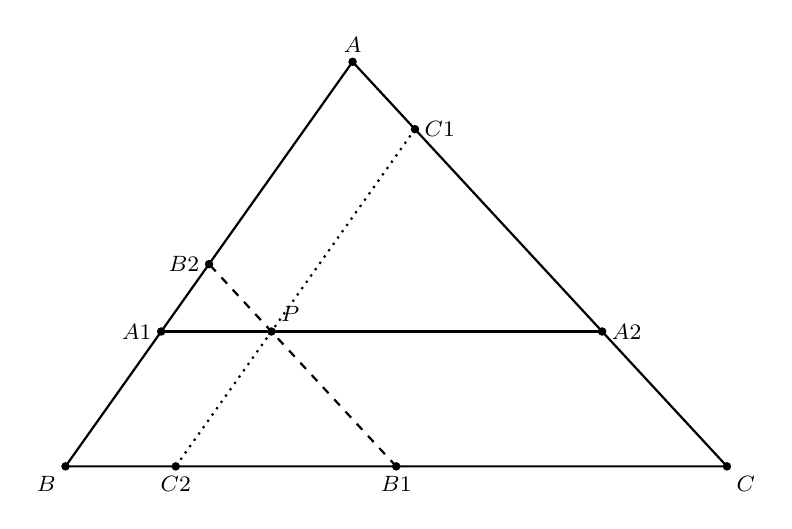
\begin{tikzpicture}[scale=0.7]
  \coordinate (B) at (0,0); \coordinate (C) at (12,0); \coordinate (A) at (5.208,7.340); \coordinate (P) at (3.736,2.447);
  \coordinate (A1) at (1.736,2.447); \coordinate (A2) at (9.736,2.447);
  \coordinate (B1) at (6,0); \coordinate (B2) at (2.604,3.670);
  \coordinate (C1) at (6.340,6.117); \coordinate (C2) at (2,0);
  \draw[thick] (A)--(B)--(C)--cycle;
  \draw[thick] (A1)--(A2); \draw[thick,dashed] (B1)--(B2); \draw[thick,dotted] (C1)--(C2);
  \foreach \p/\pos in {A/above,B/below left,C/below right,B1/below,C2/below,A1/left,A2/right,B2/left,C1/right}{\fill (\p) circle (2.2pt) node[\pos]{\footnotesize$\p$};}
  \fill (P) circle (2.2pt) node[above right]{\footnotesize$P$};
\end{tikzpicture}
\end{center}
\begin{enumerate}
  \item Soit $h$ la hauteur issue de $A$ et $d$ la distance de $P$ à $(BC)$. Montrer que $\dfrac{\ell_a}a=1-\dfrac dh$.
  \item On pose $\alpha=\dfrac{\text{aire}(PBC)}{\mathcal S}$, $\beta=\dfrac{\text{aire}(PCA)}{\mathcal S}$ et $\gamma=\dfrac{\text{aire}(PAB)}{\mathcal S}$. Montrer que $\dfrac dh=\alpha$ et que $\alpha+\beta+\gamma=1$.
  \item En déduire que $\dfrac{\ell_a}a+\dfrac{\ell_b}b+\dfrac{\ell_c}c=2$.
  \item Application : $a=12$, $b=10$, $c=9$, $\ell_a=8$ et $\ell_b=5$. Calculer $\ell_c$.
  \item Le triangle est équilatéral de côté $s$. Montrer que $\ell_a+\ell_b+\ell_c=2s$ pour tout point $P$ intérieur. Que vaut $\ell_a$ lorsque $P$ est le centre du triangle ?
\end{enumerate}

% ---SOLUTION---
\begin{prop}[Thalès et aire]
$A_1\in[AB]$, $A_2\in[AC]$ et $(A_1A_2)\parallel(BC)$ : on part de $A$, \ib{$\dfrac{AA_1}{AB}=\dfrac{AA_2}{AC}=\dfrac{A_1A_2}{BC}$}.

Aire d'un triangle : \ib{$\dfrac12\times\text{base}\times\text{hauteur}$}.
\end{prop}
\begin{enumerate}
  \item Soit $H$ le pied de la hauteur issue de $A$ ; la droite $(AH)$ coupe $(A_1A_2)$ en $K$. Les droites $(A_1A_2)$ et $(BC)$ sont parallèles et $P\in(A_1A_2)$ : $KH=d$, et $K$ est entre $A$ et $H$ (car $P$ est intérieur au triangle). Donc
  \[AK=AH-KH=h-d\]
  \textbf{Thalès de sommet $A$ dans $ABC$} :
  \[\dfrac{AA_1}{AB}=\dfrac{A_1A_2}{BC}=\dfrac{\ell_a}a\]
  \textbf{Thalès de sommet $A$ dans $ABH$} ($A_1\in[AB]$, $K\in[AH]$, $(A_1K)\parallel(BH)$) :
  \[\dfrac{AA_1}{AB}=\dfrac{AK}{AH}=\dfrac{h-d}h\]
  Les deux rapports sont égaux à $\dfrac{AA_1}{AB}$ :
  \[\dfrac{\ell_a}a=\dfrac{h-d}h=\ib{$1-\dfrac dh$}\]

  \item On calcule les deux aires avec la même base $BC=a$ :
  \[\text{aire}(PBC)=\dfrac12\,a\,d\qquad\mathcal S=\dfrac12\,a\,h\]
  \[\alpha=\dfrac{\frac12\,a\,d}{\frac12\,a\,h}=\ib{$\dfrac dh$}\]
  Comme $P$ est à l'intérieur du triangle, les triangles $PBC$, $PCA$ et $PAB$ \textbf{recouvrent} $ABC$ sans se chevaucher :
  \[\text{aire}(PBC)+\text{aire}(PCA)+\text{aire}(PAB)=\mathcal S\implies\ib{$\alpha+\beta+\gamma=1$}\]

  \item Le même raisonnement, avec le sommet $B$ puis le sommet $C$, donne
  \[\dfrac{\ell_b}b=1-\beta\qquad\dfrac{\ell_c}c=1-\gamma\]
  Avec $\dfrac{\ell_a}a=1-\alpha$ :
  \[\dfrac{\ell_a}a+\dfrac{\ell_b}b+\dfrac{\ell_c}c=3-(\alpha+\beta+\gamma)=3-1=\ib{$2$}\]

  \item On calcule les deux premiers rapports :
  \[\dfrac{\ell_a}a=\dfrac8{12}=\dfrac23\qquad\dfrac{\ell_b}b=\dfrac5{10}=\dfrac12\]
  La question 3 donne
  \[\dfrac{\ell_c}c=2-\dfrac23-\dfrac12=\dfrac{12-4-3}6=\dfrac56\]
  \[\ell_c=\dfrac56\times9=\ib{$\dfrac{15}2=7{,}5$}\]
  (On a $\alpha=\dfrac13$, $\beta=\dfrac12$ et $\gamma=\dfrac16$ : trois nombres positifs de somme $1$, donc un tel point $P$ existe.)

  \item Si $a=b=c=s$, la question 3 donne
  \[\dfrac{\ell_a+\ell_b+\ell_c}s=2\implies\ib{$\ell_a+\ell_b+\ell_c=2s$}\]
  Le centre du triangle équilatéral est à la même distance des trois côtés : les triangles $PBC$, $PCA$, $PAB$ ont même aire, donc $\alpha=\beta=\gamma=\dfrac13$.
  \[\dfrac{\ell_a}s=1-\dfrac13=\dfrac23\implies\ell_a=\ib{$\dfrac{2s}3$}\]
\end{enumerate}
\textbf{Idée :} chaque parallèle coupe le triangle dans le rapport $1-\alpha$ (resp. $1-\beta$, $1-\gamma$), et les trois aires $\alpha$, $\beta$, $\gamma$ recouvrent le triangle.

\textbf{Piège :} confondre $\dfrac{\ell_a}a$ avec $\alpha$ : le rapport de la parallèle est $1-\alpha$, pas $\alpha$.
